%\textit{D'après ressources de Quentin Fortier}

\section*{Définitions}
Soit $G = (V, E)$ un graphe non-orienté, où $V$ est un ensemble de sommets et $E$ un ensemble d’arêtes. Soit $k\in\mathbb{N}^*$. Un
$k$-coloriage de $G$ est une fonction $c : V \mapsto \{0, ..., k - 1\}$ telle que :
$\{u, v\} \in E\Rightarrow c(u) \neq c(v)$.

Dit autrement, un $k$-coloriage donne une couleur (qu’on suppose être un entier entre 0 et $k-1$, pour simplifier) à chaque sommet,
tel que deux sommets adjacents soient de couleurs différentes.
Suivant les questions, on utilisera soit une matrice d’adjacence, soit une liste d’adjacence. Attention à ne pas les confondre.
Soit $G_1$ le graphe suivant.
\begin{center}
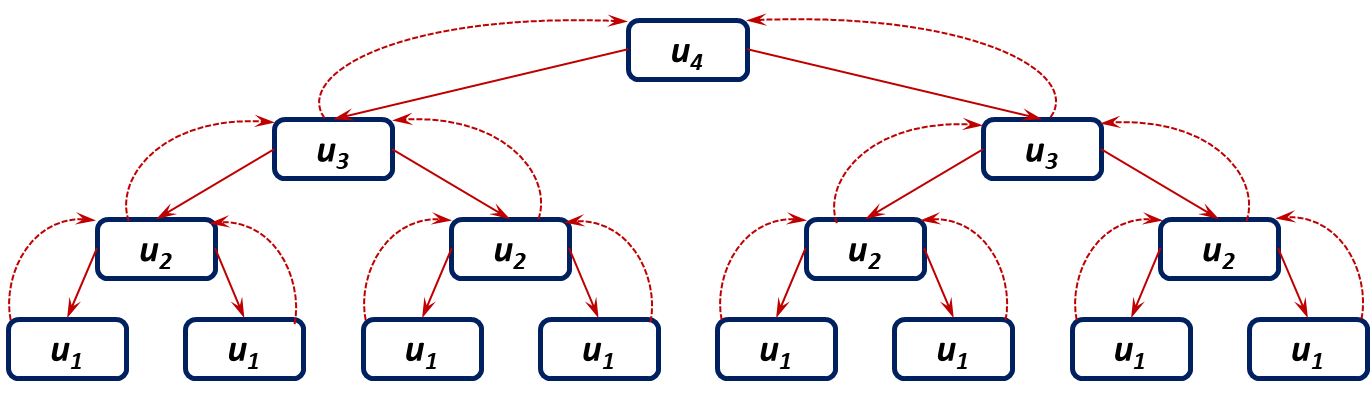
\includegraphics[width=5cm]{fig_01}
\end{center}

\question{Écrire une ou plusieurs instruction(s) Python pour définir $G_1$ par liste d’adjacence.}

\question{Donner une 3-coloration pour $G_1$. On pourra recopier $G_1$ en mettant, à côté de chaque sommet, une couleur (c’est-à-dire
0, 1 ou 2).}

\question{Justifier que $G_1$ ne possède pas de 2-coloration.}

\question{Si $n$ est le nombre de sommets d’un graphe $G$, montrer que $G$ possède une $n$-coloration.}
Dans toute la suite, on représente une $k$-coloration par une liste \lstinline{C} telle que \lstinline{C[i]} est la couleur (entre \lstinline{0} et \lstinline{k - 1})
du sommet \lstinline{i}.

\question{Écrire une fonction \lstinline{valid(G, C)} déterminant si la coloration \lstinline{C} est valide sur le graphe représenté par la liste d’adjacence \lstinline{G}.}

Par exemple, si \lstinline{G1} est la liste d’adjacence de $G_1$, \lstinline{valid(G1, [0, 0, 1, 2, 3, 4])} doit renvoyer \lstinline{False} (car les sommets
0 et 1 sont adjacents et sont tous les deux coloriés avec la couleur 0) mais \lstinline{valid(G1, [3, 0, 1, 0, 3, 4])} doit renvoyer
\lstinline{True} (toutes les arêtes ont bien des extremités de couleurs différentes).



\section*{Degré}
\question{Écrire une fonction \lstinline{deg(G, v)} renvoyant le degré d’un sommet dans le graphe \lstinline{G} représenté par liste d’adjacence.}

\question{Écrire une fonction \lstinline{deg\_max(G)} calculant le degré maximum d’un sommet dans le graphe \lstinline{G} représenté par liste d’adjacence. On appelle $\Delta(G)$ ce nombre.}

Il existe un algorithme simple donnant une $(\Delta(G) + 1)$-coloration pour un graphe $G$ : considérer chaque sommet $v$ un par un
(de 0 à $n - 1$, où $n$ est le nombre de sommets) et lui donner la plus petite couleur n’apparaissant pas parmi les voisins de $v$.

\question{Écrire une fonction \lstinline{delta\_color(G)} renvoyant une $(\Delta(G) + 1)$-coloration de \lstinline{G} représenté par matrice d’adjacence. Le
résultat sera donc une liste \lstinline{C} telle que \lstinline{C[v]} est la couleur donnée à \lstinline{v}.}

\section*{Clique}
Une clique d’un graphe \lstinline{G} est un sous-graphe complet, c’est-à-dire un ensemble de sommets contenant toutes les arêtes possibles
entre deux sommets. La taille d’une clique est son nombre de sommets.
Par exemple, l’ensemble de sommets \{1, 2, 5\} forme une clique de taille 3 de $G_1$, puisque ces 3 sommets sont tous reliés par des
arêtes.

\question{Soit $k \in \mathbb{N}^*$. Montrer que s’il existe une clique de taille $k$ dans $G$, alors $G$ n’est pas $(k - 1)$-coloriable.}

\question{Écrire une fonction \lstinline{is\_clique(G, V)} déterminant si la liste des sommets \lstinline{V} forme une clique dans la matrice d’adjacence
\lstinline{G}, c’est-à-dire si tous les sommets de \lstinline{V} sont reliés 2 à 2.}

Par exemple, si \lstinline{G1} est la matrice d’adjacence de \lstinline{G1}, \lstinline{is\_clique(G1, [1, 2, 5])} doit renvoyer \lstinline{True} mais \lstinline{is\_clique(G1, [1, 2, 3])} doit renvoyer \lstinline{False}.

\section*{2-coloration par parcours en profondeur}
On veut écrire un algorithme pour obtenir une 2-coloration d’un graphe connexe $G$. Pour cela, on exécute un parcours en
profondeur depuis un sommet $v$ quelconque (par exemple le sommet 0) de $G$, que l’on colorie avec la couleur 0, puis on colorie
les voisins de $v$ avec la couleur 1, puis les voisins des voisins avec la couleur 0...
On pourra utiliser le fait que si $c\in\{0, 1\}$ est une couleur, alors $1- c$ est l’autre couleur ($1 -c = 1$ si $c = 0$ et $1 - c = 0$ si $c = 1$).
Si, à un moment de l’algorithme, on doit colorier un sommet avec une couleur alors qu’il a déjà été colorié d’une couleur différente,
$G$ n’est pas 2-coloriable.

On stockera le coloriage dans une liste \lstinline{C} (comme pour la première partie) qui sera aussi utilisée pour savoir si un sommet a déjà été
visité.

\question{Compléter le code suivant pour renvoyer un 2-coloriage dans le graphe $G$ représenté par liste d’adjacence. Si $G$ n’a pas de
2-coloriage, on renverra \lstinline{False}.}
\begin{lstlisting}
def 2_color(G):
    # définir une liste C donnant un coloriage pour chaque sommet, avec initialement que des -1
    def aux(v, c): # parcours en profondeur sur v, en lui donnant la couleur c
        # Si v a déjà la couleur 1 - c, renvoyer False
        # Si v a déjà la couleur c, renvoyer True
        # Mettre la couleur c dans C[v]
        # Appeler récursivement aux(w, 1 - c) pour chaque w voisin de v.
        # Si un de ces appels renvoie False, renvoyer False aussi. Sinon, renvoyer True.
    # Appeler aux(0, 0). Si cela renvoie False, renvoyer False. Sinon, renvoyer C
\end{lstlisting}

\question{Si le graphe n’est pas connexe, il faut appliquer l’algorithme précédent sur chaque composante connexe. Modifier la fonction
précédente pour le faire.}


\section*{Comptage du nombre de couleurs}    
Étant donnée une liste d’entiers (des couleurs), non forcément consécutifs, on veut savoir quel est le nombre d’entiers différents
(le nombre de couleurs). Par exemple, le nombre de valeurs différentes de \lstinline{[1, 4, 0, 4, 1]} est 3 (il y a 3 entiers différents :
0, 1, 4). Pour cela, on étudie trois méthodes différentes (et indépendantes).

\question{Écrire une fonction \lstinline{ncolor1(C)} renvoyant le nombre d’entiers différents dans une liste \lstinline{C}, en utilisant 2 boucles \lstinline{for}. On pourra traduire le pseudo-code suivant en Python.}

\begin{lstlisting}
def ncolor1(C):
    L = [] # L va contenir les différentes valeurs de C
    # Pour tout élément c de C
        # Si c n'appartient pas à L
            # Alors ajouter c à L
    # Renvoyer la taille de L
\end{lstlisting}

\question{Quelle est la complexité de \lstinline{ncolor1(C)}, en fonction de la taille $n$ de \lstinline{ C} ?}    

Si \lstinline{L} est une liste, \lstinline{L.sort()} permet de trier les éléments de \lstinline{L} (par ordre croissant). \lstinline{L.sort()} modifie \lstinline{L} (mais ne renvoie
pas de valeur). On admet que \lstinline{L.sort()} est en complexité $\mathcal{O}(n \log(n))$, où $n$ est le nombre d’éléments de \lstinline{L}.

\question{Écrire une fonction \lstinline{ncolor2(C)} renvoyant le nombre d’entiers différents dans une liste \lstinline{C}, en triant \lstinline{C}. Cette fonction doit
être en complexité $\mathcal{O}(n \log(n))$ où $n$ est la taille de \lstinline{C}, et on demande de justifier cette complexité.}

Une 3ème méthode consiste à utiliser une liste \lstinline{B} de booléens de taille $p$, où $p$ est le maximum de \lstinline{C}, telle que \lstinline{B[i]} vaut
\lstinline{True} si et seulement si \lstinline{i} est dans \lstinline{C}.

\question{Écrire une fonction \lstinline{ncolor3(C)} renvoyant le nombre d’entiers différents dans une liste \lstinline{C}, en créant et utilisant une telle
liste \lstinline{B}. \lstinline{ncolor3(C)} doit être en complexité $\mathcal{O}(n + p)$ et on justifiera cette complexité.}